
%(BEGIN_QUESTION)
% Copyright 2011, Tony R. Kuphaldt, released under the Creative Commons Attribution License (v 1.0)
% This means you may do almost anything with this work of mine, so long as you give me proper credit

Suppose this feedforward control system was just recently installed on a heat exchanger, complete with ``gain'' and ``bias'' functions to allow the feedforward action to be adjusted:

$$\includegraphics[width=15.5cm]{i02462x01.eps}$$

After tuning the flow and temperature controllers (in that order), the instrument technician's next step is to place the temperature controller in manual mode, then slightly close the hand valve leading into the heat exchanger in order to introduce a load change.  The result is this trend of outlet temperature:

$$\includegraphics[width=15.5cm]{i02462x02.eps}$$

What should be adjusted in the feedforward system in order to achieve better load compensation?  Why was it important for the technician to first place the temperature controller in manual mode before attempting the load change test?  Would it have been equivalent to place the flow controller in manual mode instead?

\vskip 20pt \vbox{\hrule \hbox{\strut \vrule{} {\bf Suggestions for Socratic discussion} \vrule} \hrule}

\begin{itemize}
\item{} Predict the effects resulting from one of the transmitters in this system failing with either a {\it high} or a {\it low} signal.
\item{} Can we tell from the results of this test whether the feedforward system requires {\it lead} or {\it lag} dynamic compensation?  If so, which form of dynamic compensation do you think this system requires?
\end{itemize}

\underbar{file i02462}
%(END_QUESTION)





%(BEGIN_ANSWER)

Right now there is too much {\it gain} in the feedforward signal path, which means the feedforward control is {\it overcompensating} for changes in feed flow.

%(END_ANSWER)





%(BEGIN_NOTES)

Placing the temperature controller in manual is essential for testing feedforward action, so that the response you see is {\it purely} due to feedforward and not feedback.

\vskip 10pt

Placing the flow controller in manual mode would have been bad to do, since doing so would freeze the steam valve in one position thereby nullifying all feedforward and all feedback control!

%INDEX% Control, strategies: feedforward

%(END_NOTES)

